%
% 第三章
%
\chapter{基于UEFI的硬盘文件安全加载策略总体设计}

%
% 3.1节
%
\section{安全漏洞分析}
UEFI环境中,加载硬盘设备上的ESP分区中的系统文件是一个十分丰富的过程,它不仅包含了UEFI系统内部的文件加载
过程,它还包含着如硬盘分区的创建、硬盘文件系统的建立、操作系统安装过程中向ESP分区内添加操作系统引导文件
BootLoader等文件的过程,以及UEFI环境中识别硬盘分区方式、识别硬盘特定分区中的文件系统并通过UEFI内部
的相同文件系统格式定义,使其完成UEFI内核与硬盘设备间的文件数据交互功能。
\par 本节将介绍硬盘文件系统的建立过程,UEFI环境中硬盘文件加载的过程,以及从硬盘硬件层面和从UEFI固件层面
两方面对硬盘文件进行攻击以达到篡改ESP分区中关键系统文件的可能性。
\subsection{硬盘文件系统建立过程分析}
在一个服务器或个人电脑上安装操作系统时,其实都经历着硬盘文件系统建立的过程\cite{chinese22}。如图3-1所示,
中建立GPT硬盘
分区格式的目的为让UEFI可识别出硬盘分区的信息,传统MBR分区格式只能由传统BIOS系统识别。为硬盘创建FAT文件
系统的目的也在于统一硬件上的数据组织形式和UEFI内存中的硬盘数据处理格式\cite{extra1}。

\begin{figure}[htb]
    % 调整图片与上文的垂直距离 %
    \vspace{0cm}   
    % 调整图片图片与中文标题、中文标题与英文标题距离 %
    \setlength{\abovecaptionskip}{0.3cm}  
    % 引用/fig/目录中的图片文件 %
	\centering
    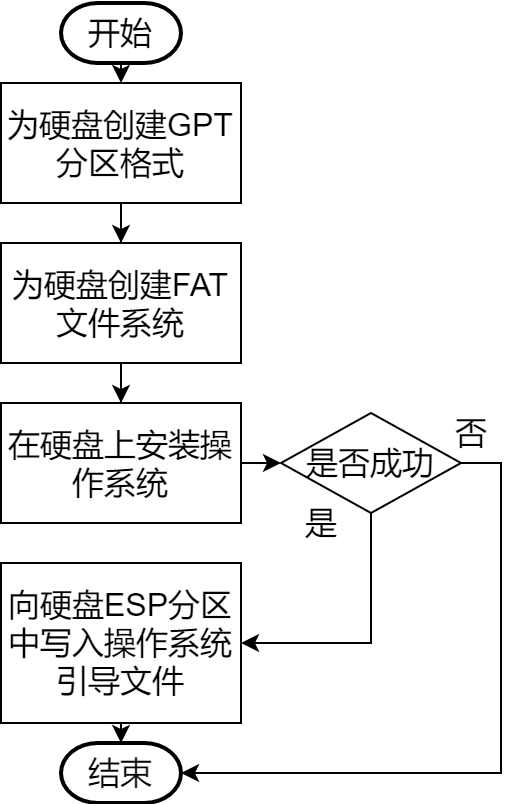
\includegraphics[width=5cm]{disk_init2.png}
    % 中文标题 %
    \caption*{图 3-1 硬盘文件系统建立过程}
    % 调整图片英文标题与下文距离(本文标准为-0.7cm) %
    \setlength{\belowcaptionskip}{-0.7cm}
    % 英文标题 %
    \caption*{Figure 3-1 Hard disk file system establishment process}
\end{figure}

而ESP分区之所以作为EFI系统分区,是因为在安装操作系统的过程中,操作系统安装程序将GPT分区格式硬盘
的其中一个分区初始化为ESP分区,并将引导加载操作系统其他模块的BootLoader引导程序等系统关键EFI程序,
放入到这个自己建立的ESP分区中。这样便有了UEFI环境中加载硬盘设备ESP分区中系统引导文件及其他关键EFI
文件的由来\cite{addition1}。

\subsubsection{服务器启动流程分析}
UEFI BIOS作为一个基础输入输出系统,为操作系统提供基础的硬件支持,同时也能引导操作体统的启动,具体
实施方式为:

\begin{figure}[htb]
    % 调整图片与上文的垂直距离 %
    \vspace{0cm}   
    % 调整图片图片与中文标题、中文标题与英文标题距离 %
    \setlength{\abovecaptionskip}{0.3cm}  
    % 引用/fig/目录中的图片文件 %
	\centering
    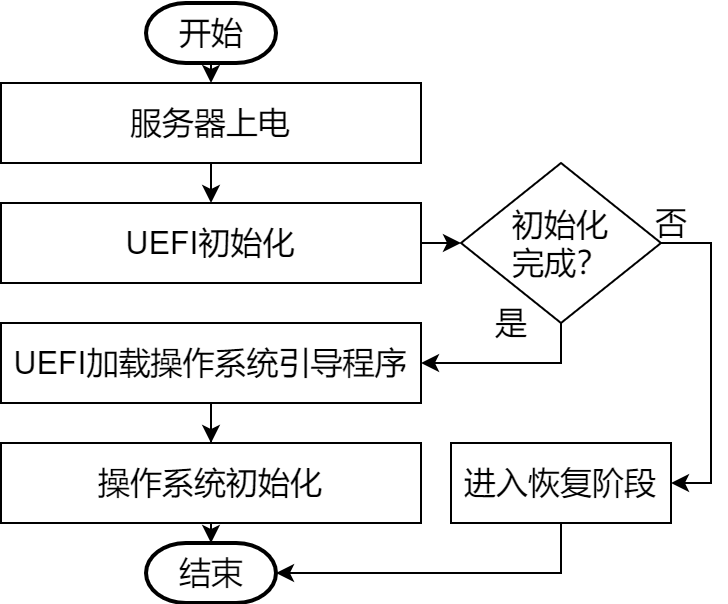
\includegraphics[width=7cm]{server_start2.png}
    % 中文标题 %
    \caption*{图 3-2 服务器启动流程}
    % 调整图片英文标题与下文距离(本文标准为-0.7cm) %
    \setlength{\belowcaptionskip}{-0.7cm}
    % 英文标题 %
    \caption*{Figure 3-2 Server startup process}
\end{figure}

如图3-2所示,服务器上电,随后初始化UEFI BIOS系统,再由UEFI系统通过内部的文件系统协议栈加载硬盘ESP
分区中的操作系统引导文件,随后控制权交给引导程序并退出UEFI系统初始化流程。

\begin{figure}[htb]
    % 调整图片与上文的垂直距离 %
    \vspace{0cm}   
    % 调整图片图片与中文标题、中文标题与英文标题距离 %
    \setlength{\abovecaptionskip}{0.3cm}  
    % 引用/fig/目录中的图片文件 %
	\centering
    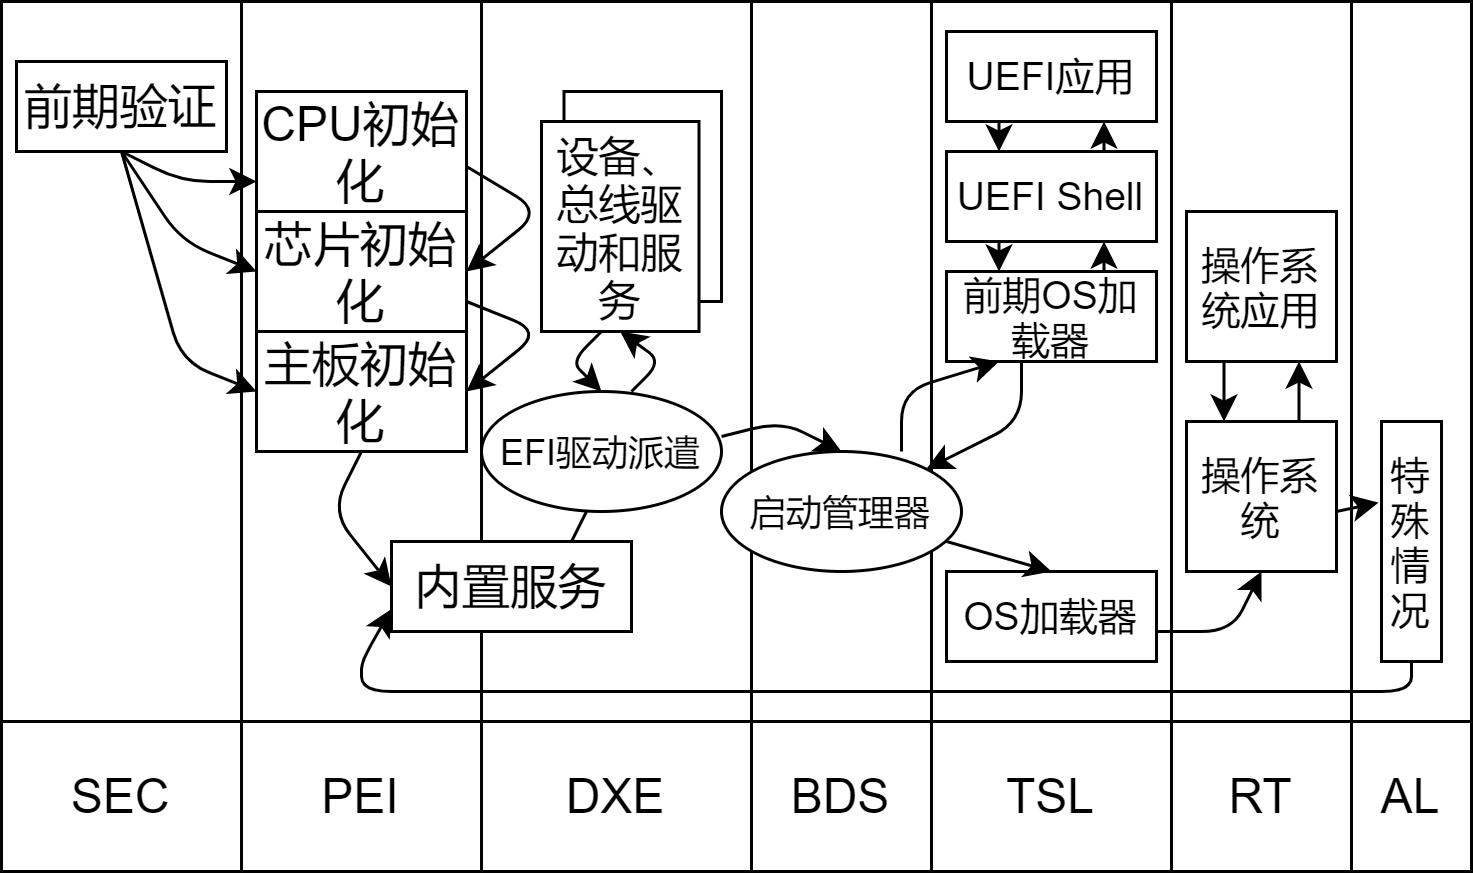
\includegraphics[width=9cm]{uefi_boot_process2.png}
    % 中文标题 %
    \caption*{图 3-3 UEFI启动流程}
    % 调整图片英文标题与下文距离(本文标准为-0.7cm) %
    \setlength{\belowcaptionskip}{-0.7cm}
    % 英文标题 %
    \caption*{Figure 3-3 UEFI boot process}
\end{figure}

本文重点研究的过程是UEFI初始化过程,和UEFI加载硬盘ESP分区文件过程。如图3-3所示,为UEFI系统的初始化流程。
如图所示,UEFI系统在遵循UEFI标准的SEC安全启动阶段后,进入PEI和DXE两个UEFI初始化阶段关键的驱动程序加载
过程,在这里完成UEFI系统的内存及内存地址的建立、硬件设备驱动程序的加载、硬件设备存储器I/O端口映射等系统
关键初始化步骤。随后通过BDS阶段的BDS core核心程序,也就是启动管理器程序,加载位于硬盘ESP分区中的前期
OS加载器以及操作系统加载器。其中,前期OS加载器用来作为SHELL用户接入程序、PXE网络启动程序等这些过程的
引导器使用;而操作系统加载器则负责引导服务器上在UEFI启动前安装的特定操作系统。

\subsection{UEFI环境文件加载过程分析}
由前面的分析可知,UEFI环境中的硬盘文件加载过程建立在硬盘块设备已经建立好GPT分区格式和与UEFI内核中对应
的文件系统格式的前提下,通过UEFI文件系统协议栈的层级关系,一层一层调用来实现硬盘文件数据加载到UEFI系统
内存的过程。

\begin{figure}[htb]
    % 调整图片与上文的垂直距离 %
    \vspace{0cm}   
    % 调整图片图片与中文标题、中文标题与英文标题距离 %
    \setlength{\abovecaptionskip}{0.3cm}  
    % 引用/fig/目录中的图片文件 %
	\centering
    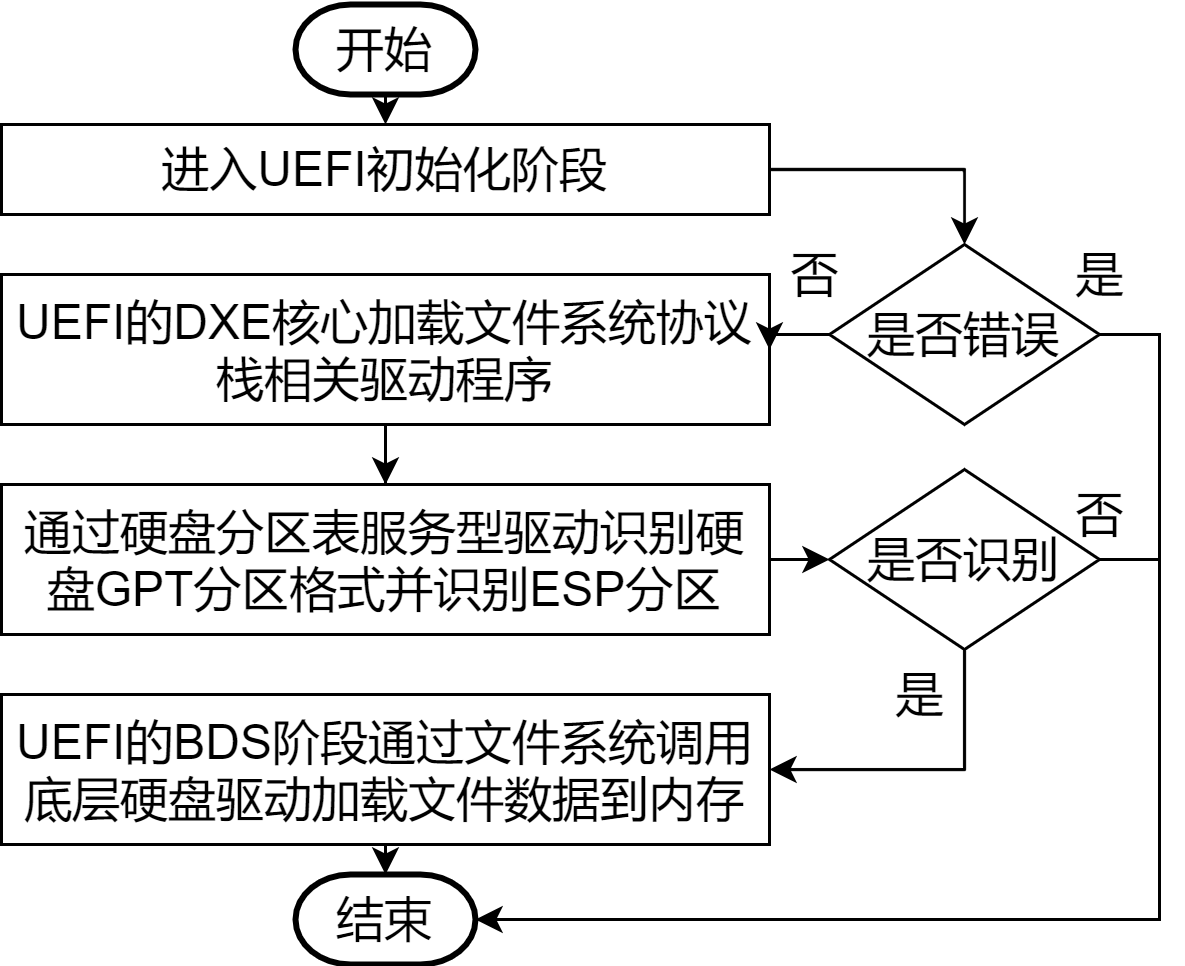
\includegraphics[width=8cm]{uefi_loadfile_process2.png}
    % 中文标题 %
    \caption*{图 3-4 UEFI文件加载过程}
    % 调整图片英文标题与下文距离(本文标准为-0.7cm) %
    \setlength{\belowcaptionskip}{-0.7cm}
    % 英文标题 %
    \caption*{Figure 3-4 UEFI load file process}
\end{figure}

如图3-4所示,UEFI会先通过DXE加载UEFI文件系统协议栈相关的驱动程序,具体驱动程序为:PassThruDxe、
PartitionDxe、DiskIoDxe、FileSysDxe四个驱动,其中PassThruDxe和FileSysDxe会根据具体系统的不同
而确定不同的特定硬盘接口和文件系统。通过加载UEFI文件系统协议栈驱动程序,UEFI内核已经完成了文件系统
协议栈的建立,包括各个驱动功能函数在UEFI永久内存中的驻留以及对应UEFI协议对特定硬盘驱动的函数引用;
再通过在DXE阶段加载的PartitionDxe硬盘分区表服务型驱动程序,识别出硬盘的GPT分区格式并获取到GPT分区
表,通过GPT分区表再得到硬盘的ESP分区的起始和结束扇区位置,从而确定UEFI内核在BDS阶段读取操作系统
引导文件的分区位置;接下来就是UEFI进入BDS阶段并通过文件系统协议栈加载硬盘ESP分区中的文件到内存中,
并移交控制权到这个EFI可运行文件身上。
\par UEFI文件系统协议栈加载硬盘文件数据的过程,从函数调用的角度看,就是上层FileIo系统调用,调用
通过FileSysDxe加载得到的UEFI内核中的文件系统,并通过文件系统调用底层的由PassThruDxe和DiskIoDxe
驱动提供的硬盘驱动程序。在UEFI环境中,驱动功能的调用通过与其对应并对其引用的协议完成。

\subsection{从硬盘攻击关键文件}
有了对前面的硬盘分区和文件系统,UEFI系统内的文件系统的建立过程和UEFI环境中文件的加载过程的了解,
可知黑客可通过硬件手段攻击位于硬盘硬件设备上的文件系统结构\cite{chinese33}、和攻击用来存储BIOS的固件芯片两方面,
来到达篡改UEFI加载硬盘文件的文件内容。

\begin{figure}[htb]
    % 调整图片与上文的垂直距离 %
    \vspace{0cm}   
    % 调整图片图片与中文标题、中文标题与英文标题距离 %
    \setlength{\abovecaptionskip}{0.3cm}  
    % 引用/fig/目录中的图片文件 %
	\centering
    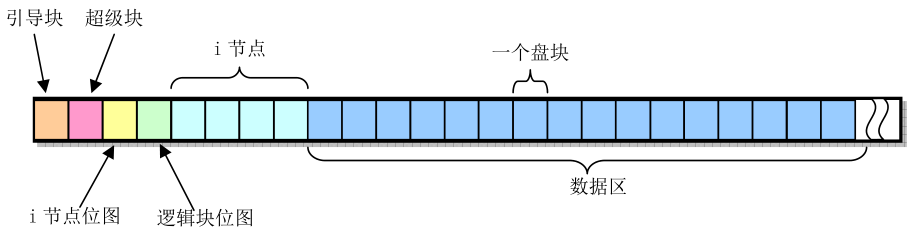
\includegraphics[width=13cm]{minix_fs_layout.png}
    % 中文标题 %
    \caption*{图 3-5 MINIX文件系统硬盘布局}
    % 调整图片英文标题与下文距离(本文标准为-0.7cm) %
    \setlength{\belowcaptionskip}{-0.7cm}
    % 英文标题 %
    \caption*{Figure 3-5 MINIX file system hard disk layout}
\end{figure}

\par 首先是针对硬盘设备的攻击,如图3-5所示,是MINIX文件系统在硬盘上的数据结构布局图\cite{chinese30},
作为一个类
UNIX文件系统,其与标准UNIX文件系统的设计结构基本相同,FAT文件系统和ext2文件系统也同样属于类UNIX
文件系统。由于各种类UNIX文件系统的基础设计理念和结构基本相同,不同之处仅在于更新一代的文件系统会
提供更为丰富的如数据恢复、文件操作日志记录等内容,而底层基础功能结构不变,因此以MINIX作为说明\cite{chinese31}。
\par 其中引导块对应于UEFI系统中硬盘的ESP分区,里面装载了操作系统所需的引导程序。超级块用于存放
盘设备上文件系统结构的信息,并说明各个部分大小。i节点位图用于说明i节点是否被使用,每个比特位代表
一个i节点。逻辑块位图用于描述盘上的每个数据盘块的使用情况,每个比特位代表盘上数据区中的一个盘块。
盘上的i节点部分存放着文件系统中文件或目录的索引节点,每个文件或目录都对应一个i节点。其中每个特定
文件对应的i节点数据结构中,都存有一个其包含的所有文件数据磁盘块的映射关系,用于通过i节点索引文件
数据。
\par 由以上分析可知,黑客可通过技术手段将恶意代码文件事先存入硬盘ESP分区或引导块中\cite{chinese32},
并获取到恶意
代码文件和UEFI将加载的系统文件分别对应的i节点,然后通过硬件手段修改i节点数据结构中文件数据块映射
的关系,将系统文件链接到恶意代码文件的数据块链,使UEFI加载系统文件时实际运行的却是恶意代码。因此
在UEFI系统中,在加载硬盘系统文件或关键文件前,对其进行完整性测量以保证加载的文件没有经过篡改,这
个过程就显得十分必要。

\subsection{从固件芯片攻击关键驱动}
作为UEFI内核与硬盘硬件设备连接的桥梁,文件系统定义了双方共同的数据组织形式和结构,来达到数据互通
的效果。因此,作为存储在BIOS固件系统上的文件系统驱动程序,同样可以作为黑客用来篡改硬盘ESP分区中
关键文件信息的攻击对象。

\begin{figure}[htb]
    % 调整图片与上文的垂直距离 %
    \vspace{0cm}   
    % 调整图片图片与中文标题、中文标题与英文标题距离 %
    \setlength{\abovecaptionskip}{0.3cm}  
    % 引用/fig/目录中的图片文件 %
	\centering
    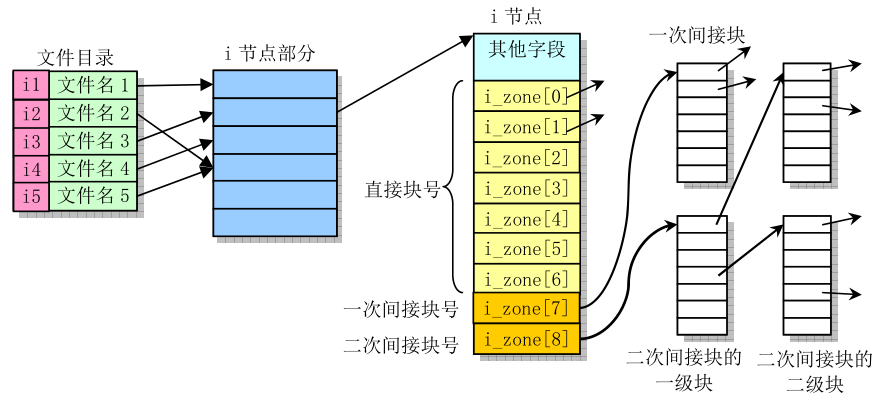
\includegraphics[width=13cm]{fs_inode_zone.png}
    % 中文标题 %
    \caption*{图 3-6 内存中的文件系统索引文件方式}
    % 调整图片英文标题与下文距离(本文标准为-0.7cm) %
    \setlength{\belowcaptionskip}{-0.7cm}
    % 英文标题 %
    \caption*{Figure 3-6 Method of index file by file system in memory}
\end{figure}

如图3-6所示,当UEFI加载了文件系统驱动之后,内存中便驻留了文件系统组织文件的方式及特定的数据结构。
当UEFI系统通过文件名索引硬盘中的文件数据时,会通过目录项这个数据结构中的i节点信息确定这个绝对路径下
特定文件名对应的硬盘中的i节点,并以此来获取到文件数据。
\par 在这个文件系统内部通过文件名检索文件数据的过程中,黑客可以通过改变文件目录项中文件名与i节点
的对应关系,来篡改特定系统文件名所对应的具体硬盘数据内容\cite{chinese15}。同样可以在内存的文件系统中,
更改i节点与
文件数据块关系,也就是更改图3-6中的i\_zone指针所指向的位置,来完成恶意代码数据对系统文件数据的更替
效果。因此,在UEFI加载文件系统模块及其相关驱动前,对他们在BIOS固件芯片中内容进行完整性度量,以确保
UEFI运行的是可信的文件系统代码,可以从固件层面消除黑客对硬盘文件内容篡改的可能。

%
% 3.2节
%
\section{信任链的设计}
在对UEFI文件系统协议栈驱动程序和硬盘ESP分区中系统关键EFI文件进行可信度量的同时,需要首先建立UEFI
系统的可信启动。根据TCG平台规范,本文选用具有存储UEFI驱动程序度量基准值功能的BMC系统作为UEFI可信
启动信任链的可信平台模块\cite{chinese5},用包含基准值存取、可信度量日志记录基本功能的BMC来作为替代传统TPM的底层
平台。

\begin{figure}[htb]
    % 调整图片与上文的垂直距离 %
    \vspace{0cm}   
    % 调整图片图片与中文标题、中文标题与英文标题距离 %
    \setlength{\abovecaptionskip}{0.3cm}
    % 引用/fig/目录中的图片文件 %
	\centering
    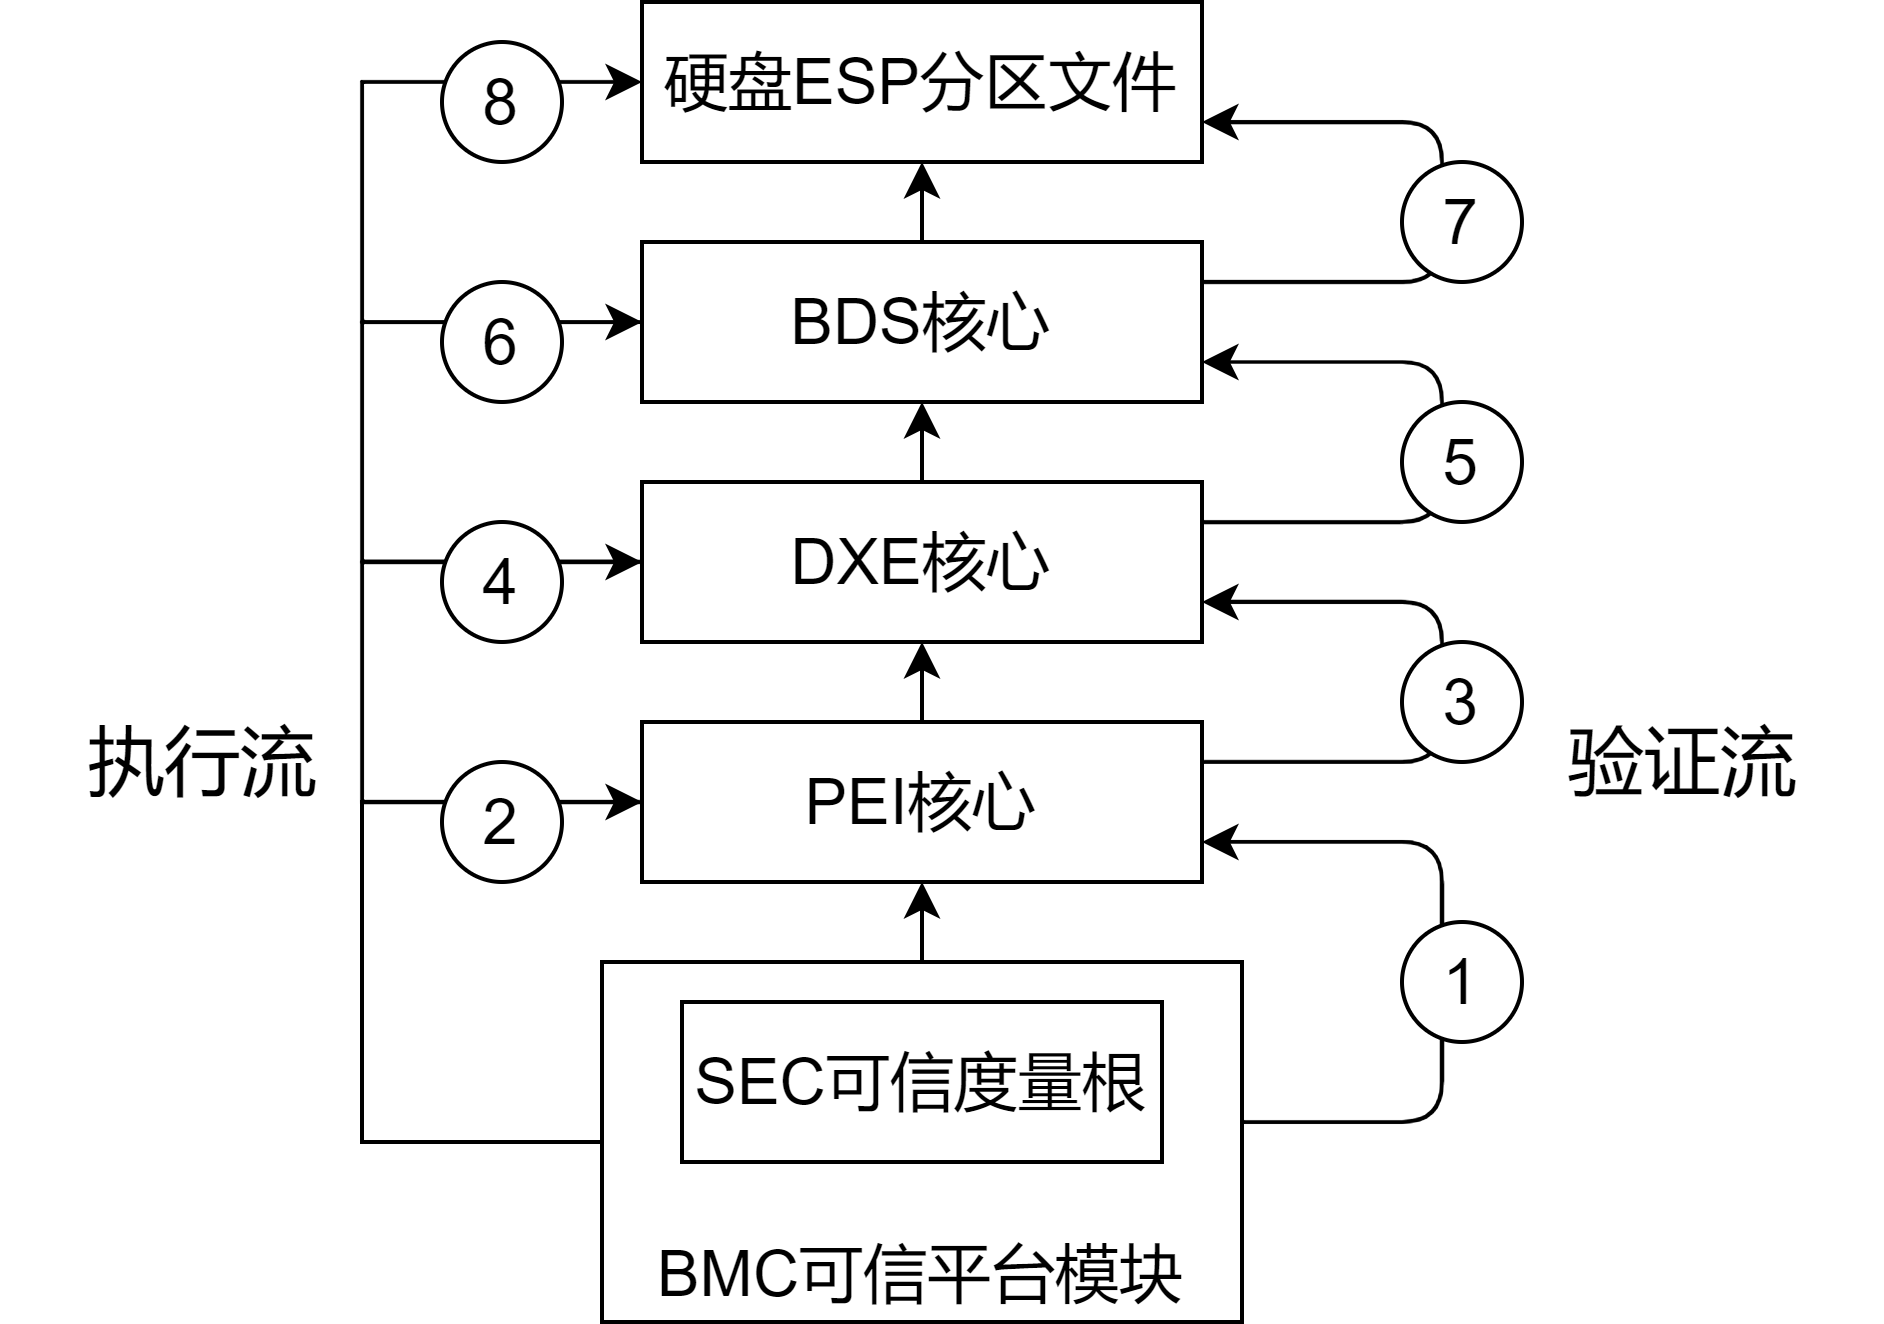
\includegraphics[width=10cm]{trust_link.png}
    % 中文标题 %
    \caption*{图 3-7 UEFI信任链传递}
    % 调整图片英文标题与下文距离(本文标准为-0.7cm) %
    \setlength{\belowcaptionskip}{-0.7cm}
    % 英文标题 %
    \caption*{Figure 3-7 UEFI trusted chain transfer}
\end{figure}

如图3-7所示,信任链以BMC系统作为可信平台模块\cite{chinese28},并以UEFI的第一阶段SEC启动
阶段作为信任链中的可信根。
然后在SEC阶段,借助BMC系统中的可信平台模块对PEI阶段的核心代码进行可信度量,在得到可信度量的结果
为PEI核心可信时,将系统控制权交给PEI核心;PEI核心借助BMC中的基准值,对系统cpu、主板和芯片组的PEIM
组件进行可信度量,并根据度量结果最后对DXE核心进行度量,并将系统控制权交给DXE核心;DXE核心阶段加载
系统其余组件,同时对UEFI文件系统协议栈的驱动程序进行度量,以保证在BDS阶段加载硬盘文件时,数据流所
经过的底层UEFI文件系统协议栈可信。最后对BDS核心进行可信度量;系统控制权交给BDS阶段核心代码,在
加载硬盘ESP分区中关键文件时,对文件内容进行度量,若可信,再将控制权交给文件进行UEFI系统调用\cite{chinese12}。

%
% 3.3节
%
\section{安全方案启动阶段设计}
根据UEFI启动阶段信任链的设计,本安全方案涉及到的UEFI启动阶段为SEC、PEI、DXE、BDS,以做到在保证
硬盘文件数据经过的硬盘设备、硬盘文件系统协议栈安全可信的同时,还要保证在BDS阶段加载硬盘文件时,
BDS核心代码的安全可信。因此安全方案分成SEC、PEI、DXE、BDS四个阶段进行设计\cite{english1},其中的DXE和
BDS阶段包含了此安全方案的主要度量内容,因此单独在下一小结进行他们和总体架构的介绍。
下面将对安全方案在SEC和PEI阶段的设计进行描述。

\subsection{SEC阶段}
SEC(Security Phase)阶段是UEFI平台初始话的第一个阶段,计算机系统加电后首先进入这个阶段。SEC阶段
首先接收并处理系统启动和重启信号,系统加电信号、系统重启信号、系统运行过程中的异常信号。还有一个重要
过程为初始化临时存储区域。系统运行在SEC阶段时,仅CPU和CPU内部资源被初始化,而各种外部设备和内存都没
有被初始化。因此系统需要一部分临时内存用于代码和数据的存储,一般称为临时RAM,临时RAM只能位于CPU内部
。最常用的临时RAM是Cache,把其当成内存使用,这种技术称为CAR(Cache As RAM)。
\par SEC阶段的目的是为PEI阶段准备一切所需的资源,包括了通过CAR得到的RAM地址和大小、栈地址和大小以及
固件卷fv的位置,使PEI可以通过这些信息加载系统资源及后续流程。本安全方案在SEC阶段的设计为,度量PEI 
core代码,得到度量结果,并判断是否将控制权由SEC传递给PEI。

\par 由于SEC阶段是此可信链中的信任根,因此SEC阶段的数据内容安全可信,又因为SEC阶段占有很少的系统资源,仅有很小的
临时内存,因此不涉及BMC的交互功能,将SEC阶段度量PEI core的基准值信息,也就是PEI core的SHA1散列值,和临时的
SHA1算法,集成在SEC core的代码中,以此来完成阶段度量的任务。SEC阶段的BMC日志信息的输出由于不借助IPMI协议,
因此不需要BMC驱动程序,只需调用上述BMC串口写入函数,即可将日志信息写入BMC芯片中。

\subsection{PEI阶段}
系统控制权到了PEI(Pre-EFI Initialization)阶段,并由PEI core核心代码负责运行PEI阶段的功能。虽然SEC
阶段对CPU和CPU内的资源进行了初始化,但是PEI阶段可用的资源依旧十分有限,该阶段对内存进行初始化,主要功
能是为DXE阶段准备执行环境,将所需要传递给DXE的信息组成HOB(Hand Off Block)列表,最终将控制权转交到DXE。
\par PEI和DXE一个不同之处在于,DXE拥有适量的系统永久RAM可供使用;而PEI仅仅拥有一些有限的临时RAM,
并且这些临时RAM在PEI阶段初始化永久内存后可能会被重新配置以作其它的用途,比如缓存(Cache)。因此,
PEI没有DXE的资源丰富。而PEI阶段的一个主要目的就是以最少的系统资源初始化永久内存,也就是UEFI系统和后面
的操作系统都可以使用的系统全部内存空间。
\par FV(Firmware Volume)的内容遵循EFI闪存文件系统的格式。PEI基础按照EFI闪存文件系统的格式来
发现FV中的PEIM。一个平台特有的PEIM可以通知PEI基础系统中的其它固件卷所处的
位置,这就允许PEI基础在其它固件卷体中找到PEIM。PEI基础和PEIM在EFI闪存文件
系统中用一个唯一的ID来命名。

\begin{figure}[htb]
    % 调整图片与上文的垂直距离 %
    \vspace{0cm}   
    % 调整图片图片与中文标题、中文标题与英文标题距离 %
    \setlength{\abovecaptionskip}{0.3cm}
    % 引用/fig/目录中的图片文件 %
	\centering
    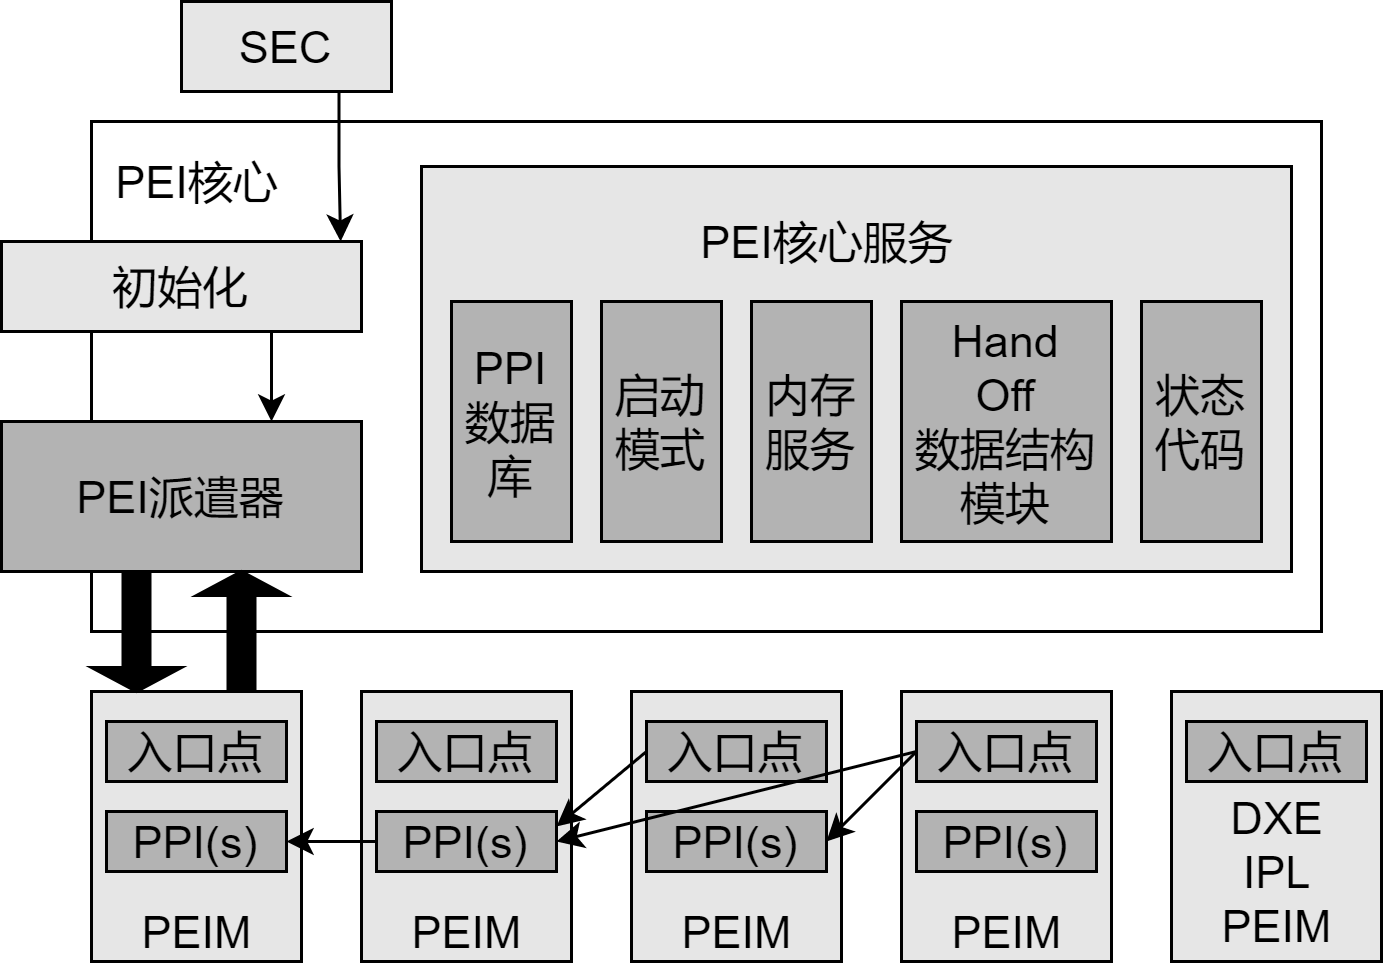
\includegraphics[width=10cm]{pei_core2.png}
    % 中文标题 %
    \caption*{图 3-9 PEI阶段系统结构}
    % 调整图片英文标题与下文距离(本文标准为-0.7cm) %
    \setlength{\belowcaptionskip}{-0.7cm}
    % 英文标题 %
    \caption*{Figure 3-9 System structure of PEI}
\end{figure}

如图3-9所示,PEI阶段的主要结构分为PEI core也就是PEI基础代码,负责PEI阶段的整体功能执行;
PEI阶段的系统服务,用于PEI阶段功能函数的调用;PEI Dispatcher调度程序,用于调用FV固件卷中
的PEIM模块,其中就包括系统最基本的cpu、主板和芯片组的PEIM。当一个PEIM调度完成之后,PEI调
度程序将继续检查固件容卷,直到出现下列两种情况之一为止:
\par (1)所有被发现的PEIM都已经被调度
\par (2)不再有PEIM可被调度
\par 这是因为任何PEIM都不能满足上述列出的调度条件。一旦达到上述两个条件中的任一个,PEI调度
程序的工作就完成了,并且它调用一个用于启动下一阶段框架的架构PPI,即DXE初始程序加载
(Initial Program Load, IPL)PPI。

\par PEI阶段的BMC通信功能的实现与DXE阶段实现过程相同,唯一不同点在于BMC驱动中的系统调用。其中PEI阶段的BMC通信模块
需要调用名为EFI\_PEI\_SERVICES的PEI阶段核心服务结构体,也就是PEI阶段的系统服务,而DXE阶段的BMC通信模块需要
调用EFI\_SYSTEM\_TABLE也就是DXE阶段的系统服务。PEI和DXE两个阶段不同的系统服务都是在过程开始阶段,通过前一
阶段传来的HOB数据结构,分别是SEC阶段和PEI阶段建立的HOB,来确定系统函数的初始化工作。由于在两个不同阶段的BMC
通信模块中,都需要使用系统函数来进行一些UEFI系统缓存的建立,因此必须要分开实现。

\begin{lstlisting}
EFI_STATUS
EFIAPI
PeiServicesLocatePpi (
    IN CONST EFI_GUID                   *Guid,
    IN UINTN                      Instance,
    IN OUT EFI_PEI_PPI_DESCRIPTOR **PpiDescriptor,
    IN OUT VOID                   **Ppi
)
\end{lstlisting}
还有一方面必须两个阶段分开实现BMC通信模块的原因在于,PEI阶段是通过PEIM安装的PPI接口来实现PEIM之间的通信,
以及PEI core对PEIM实现的功能函数的调用,通过上面的代码把以通过加载PEIM安装到系统的PPI找到,并存放在**PPI
指针中。而DXE阶段则是通过Protocol来进行驱动函数的安装及调用。PPI的安装和查找调用也是通过EFI\_PEI\_SERVICES
来进行系统调用实现的。

%
% 3.4节
%
\section{总体架构设计}
此安全方案中对四种UEFI文件系统协议栈驱动程序的度量过程和硬盘ESP分区中关键文件的度量过程是在DXE和BDS阶段
完成的,因此这两个阶段包含了此安全方案的总体架构设计内容,具体内容如下所示。图3-13展示了此安全方案在
DXE阶段的总体功能设计。

\begin{figure}[htb]
    % 调整图片与上文的垂直距离 %
    \vspace{0cm}   
    % 调整图片图片与中文标题、中文标题与英文标题距离 %
    \setlength{\abovecaptionskip}{0.3cm}
    % 引用/fig/目录中的图片文件 %
	\centering
    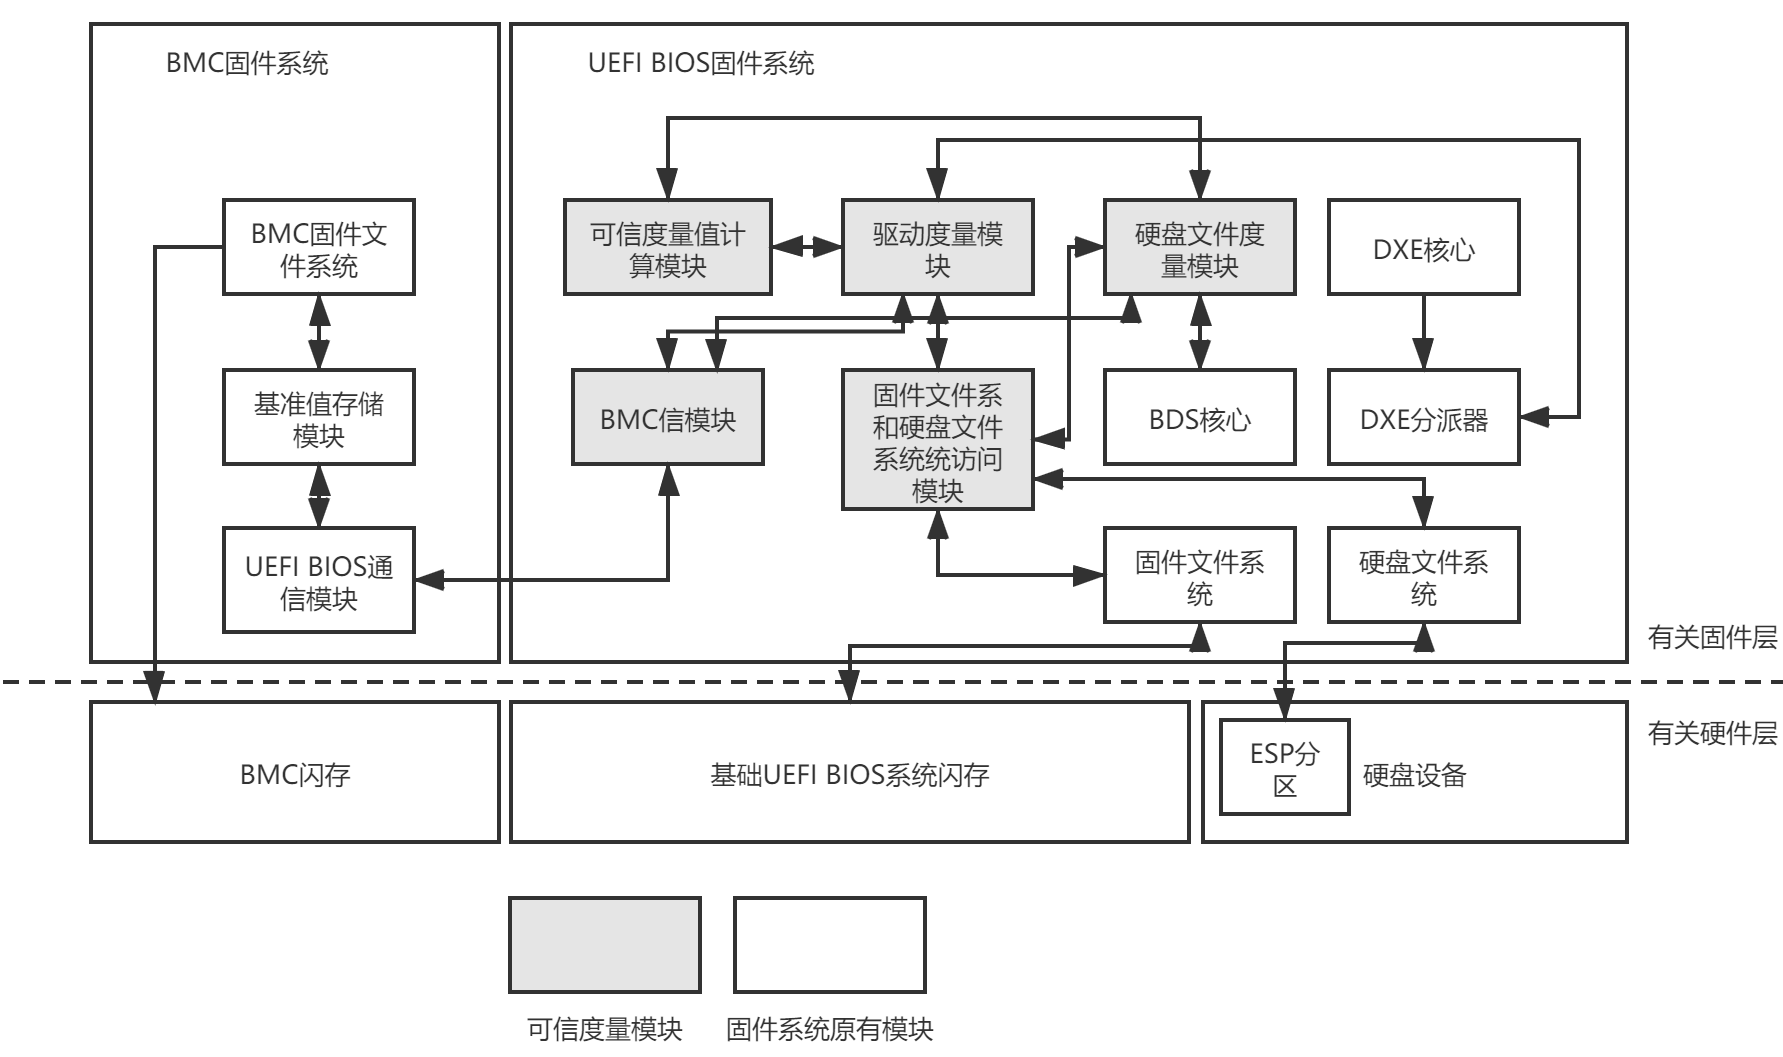
\includegraphics[width=14cm]{system_framework.png}
    % 中文标题 %
    \caption*{图 3-13 系统结构图}
    % 调整图片英文标题与下文距离(本文标准为-0.7cm) %
    \setlength{\belowcaptionskip}{-0.7cm}
    % 英文标题 %
    \caption*{Figure 3-13 System framework}
\end{figure}

如图3-13所示,此系统涉及到用来存储各个阶段核心程序和文件系统协议驱动程序的基准值的BMC固件系统,而
此安全方案中的可信度量模块以DXE驱动程序的形式,存储于UEFI BIOS固件芯片中,并通过UEFI系统原有的
DXE core和DXE调度程序加载可信度量驱动至内存中。
\par 在度量过程中,由DXE阶段的调度程序给可信度量驱动中的驱动度量模块发送度量信号,由驱动度量模块
通过文件系统协议栈驱动的全局唯一标识信息匹配出四个驱动程序,并通过UEFI中的固件文件系统FFS获取到存储
于FV固件芯片中的驱动程序数据到UEFI内存,并调用可信度量值计算模块计算出FV中驱动的hash值;再调用BMC
通信模块,通过GUID获取到存储于BMC芯片中的度量基准值,通过驱动度量模块对基准值和度量值的比较得到度量
结果。
\par 到了BDS阶段,在BDS core加载硬盘文件前,通过调用硬盘文件度量模块负责调度其他可信度量模块,具体
过程和驱动度量模块相同,不同之处在于,所获得的硬盘数据文件需要通过UEFI文件系统协议栈加载存储于硬盘
ESP分区中的关键文件,并进行度量获得度量结果。下面将对每个功能模块的设计和完成的内容进行介绍。

\par (1)驱动度量模块
\par 此模块负责通过固件文件系统FFS从UEFI BIOS flash芯片中加载AtaAtapiPassThruDxe、PartitionDxe、
DiskIoDxe、FileSystemDxe驱动代码得到各个驱动在内存中对应的内存映像Image(下同)的基地址和Image大小,
从而得到各个驱动的数据内容。其中获取flash芯片中数据过程通过调用固件文件系统访问模块完成。并通过BMC通信
模块获取基准值,存储于基准值缓存模块中。此模块中通过调用动态可信度量值计算模块计算驱动的SHA1值,并在驱
动文件可信度量顺序映射模块中进行对比得到验证结果。

\par (2)硬盘文件度量模块
\par 此模块通过UEFI环境中的文件系统协议栈调用关系,调用硬盘文件系统访问模块提取硬盘位于ESP分区中的关键
文件数据start\_kernel.efi文件,并通过调用动态可信度量计算模块计算此文件的SHA1值,由动态可信度量计算模块
将此start\_kernel.efi文件基准值返回给驱动文件可信度量顺序映射模块并存储在这个模块中。然后通过BMC通信模块
获取此文件基准值,返回的结果存储于此模块中。

\par (3)可信度量值计算模块
\par 动态可信度量值计算模块,此模块通过在固件编译时加载进去的opensslpkg包中的安全相关SHA1功能函数,
对驱动文件可信度量顺序映射模块中的四个UEFI文件系统协议栈驱动程序AtaAtapiPassThruDxe、PartitionDxe、
DiskIoDxe、FileSystemDxe的内容进行SHA1值计算,以获取运行过程中的驱动度量值,用以和基础性BMC固件系
统中的基准值存储模块中存入的基准值比对。

\par (4)固件文件系统和硬盘文件系统访问模块
\par 此模块通过判断传入的访问请求,确定需要访问固件文件系统内数据或硬盘数据。其中访问固件中文件数据过程
中,此模块封装了UEFI服务提供的访问固件文件系统FFS的功能函数,将文件系统协议栈相关驱动程序加载进UEFI系统内
存中。访问硬盘数据过程中,此模块通过使用UEFI文件系统协议栈内容,并调用最上层FileIo
协议,读取硬盘设备中的关键文件数据到UEFI系统内存中。

\par (5)BMC通信模块
\par 此模块负责实现BMC的UEFI驱动程序,其中通信协议为IPMI协议,访问模式遵循KCS方式,实现向BMC发送IPMI格式
的命令信息,并实现获取BMC返回基准值的函数。从而实现UEFI环境中与BMC设备通信的功能,完成可信度量模块中获取基
准值的工作。

%
% 3.5节
%
\section{本章小结}
本章首先对UEFI系统加载硬盘ESP分区中文件数据的过程进行了分析,通过对文件系统数据组织结构的分析找出
了文件加载过程中的安全漏洞,并针对通过UEFI文件系统协议栈加载硬盘数据的过程,划分了UEFI启动不同阶段
中的安全方案,并提出了DXE阶段和BDS阶段所涉及到的可信度量驱动和相关模块的调用关系及BMC系统存储基准值
的作用,为后文安全方案的具体实施奠定了基础。

\bjutclearpage
